\apendice{Documentación técnica de programación}

\section{Introducción}

En este apartado se va a describir la documentación técnica referente a la programación. Se incluirá la preparación del entorno de desarrollo utilizado y la estructura de la aplicación.

\section{Estructura de directorios}

El proyecto tiene la siguiente estructura de directorios:

\begin{itemize}
	\item 
	\textbf{/Aplication/:} Contiene los siguientes elementos:   
		\begin{itemize}
		\item Ejecutable \textbf{\emph{SIM.exe}:} Haciendo doble clic sobre el ejecutable se ejecuta la aplicación.
		\item Carpeta \textbf{\emph{/Aplication/img}:} Contiene las imágenes que se utilizan en la interfaz gráfica.
		\item \textbf{\emph{about.pdf}:} \emph{Acerca de...} de la interfaz gráfica.
		\item  \textbf{\emph{ayuda.pdf}:} \emph{Ayuda Local} de la interfaz gráfica.
		\item  \textbf{\emph{BBDD}:} Base de Datos ya creada de la aplicación con un conjunto de datos introducidos. Este fichero se puede crear con la aplicación, pero se suministra para probar la misma.
		\item  \textbf{\emph{ficheroSigma.xls}:} Fichero descargado de la aplicación {Sigma} para que pueda ser usado como fichero de entrada de nuestra aplicación.
		\item  \textbf{\emph{ficheroSigma2.xls}:} Otro ejemplo similar al anterior.
		
		\end{itemize}
	\item 
	\textbf{/Code/:} En esta carpeta se encuentra los ficheros \emph{SIM.py} y \emph{SIM.ipynb} donde se hayan todas las funcionalidades programadas del proyecto.
	
	\item 
	\textbf{/Documentation/:} Contiene todos los ficheros relacionados con la documentación del proyecto.
			
			\begin{itemize}
			\item \textbf{Memoria.pdf:} Documento que contiene la memoria del proyecto. 			
	
			\item \textbf{Anexos.pdf:} Documento que contiene los anexos del proyecto.
			
			\item \textbf{/Documentation/tex:} Contiene todos los apartados en los que se desglosa tanto la memoria como los anexos.
			\item \textbf{/Documentation/img:} Contiene todas las imágenes utilizadas en la memoria y en los anexos.
			\end{itemize}
	
	\item 
	\textbf{/:} Contiene un fichero \emph{GitHub\_Repository\_Link.txt} que contiene el enlace al repositorio del proyecto de \emph{GitHub}, un fichero \emph{SIM.mp4} que es un vídeo de demostración de uso de la aplicación y un fichero \emph{README.txt} que contiene una serie de indicaciones, así como la licencia.
	
\end{itemize}

\section{Manual del programador}

Esta sección, tiene como objetivo principal, servir de punto de partida o referencia para futuras personas que decidan mejorar la aplicación.
Se va a explicar cómo se han instalado las herramientas principales para el desarrollo del proyecto, así como la compilación y ejecución del mismo. También se explicará como obtener el código y ficheros necesarios.



\begin{itemize}
			\item \textbf{Anaconda Navigator.} \emph{Anaconda} ha sido la opción utilizada para poder utilizar \emph{Juypter Notebook}\footnote{\href {https://jupyter.org/}{www.jupyter.org}} en la versión 5.7.4 como entorno de desarrollo principal.
			\emph{Anaconda Navigator} es una plataforma completamente gratuita, y podemos descargarla a través del siguiente enlace 
\footnote{\href {https://www.anaconda.com/distribution/ }{www.anaconda.com/distribution}}.
Antes de descargarlo, deberemos seleccionar la opción de \emph{Python 3.7 version}, ya que es la versión que se ha utilizado para el desarrollo del proyecto.

La instalación de la plataforma no tiene ninguna dificultad, pero si hubiera algún inconveniente, en Internet existen numerosos vídeos explicativos de cómo realizar la descarga paso a paso.

Una vez instalada, abrimos la aplicación y veremos una pantalla similar a la figura \ref{fig:jupyter}. Seleccionamos \emph{Jupyter Notebook} y ya tendríamos listo la plataforma de desarrollo. 

\begin{figure}%[!h]
		\centering
		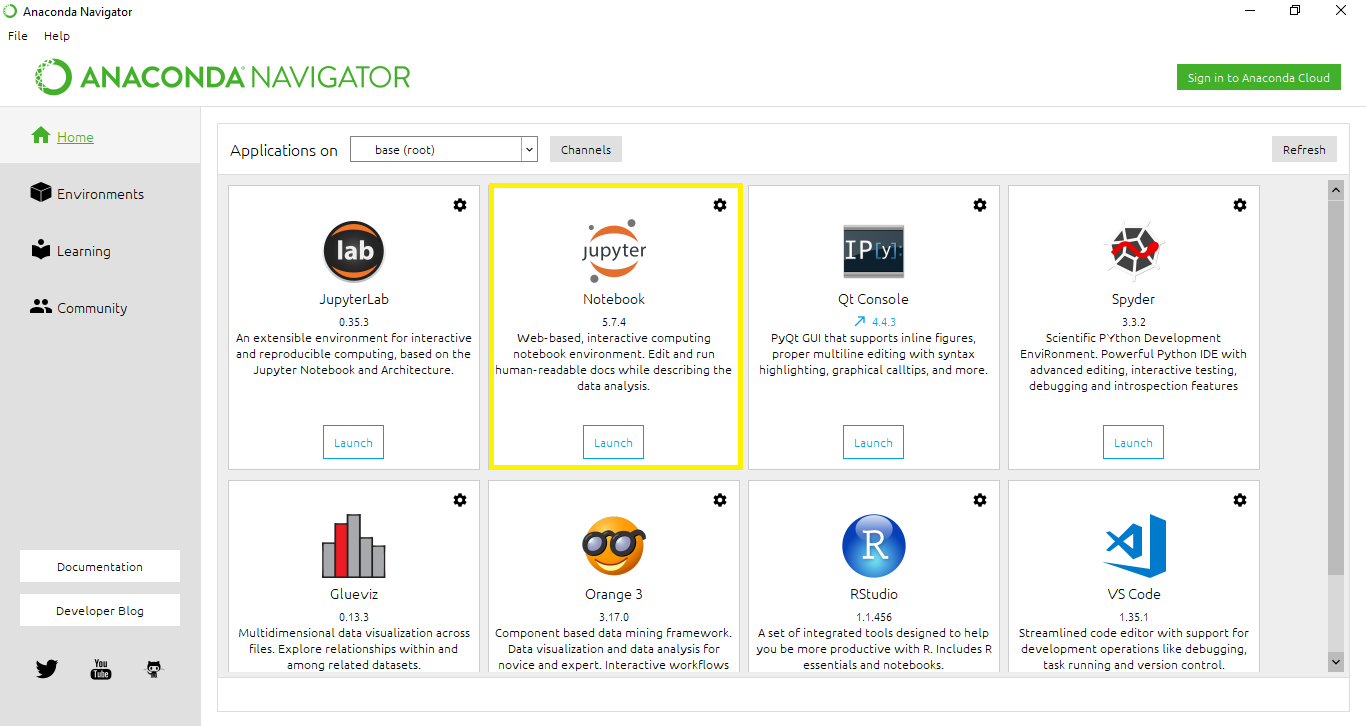
\includegraphics[width=1.1\textwidth]{jupyter}
		\caption{Anaconda Navigator}\label{fig:jupyter}
	\end{figure} 			
			
			\item \textbf{Bibliotecas o librerías utilizadas.} No se necesita la instalación de ninguna de las librerías utilizadas, ya que todas vienen incluidas en la plataforma anteriormente descargada (\emph{Anaconda Navigator}).
			
		
			\item \textbf{DB Browser.} Como se ha comentado en la memoria, DB Browser\footnote{\href{https://sqlitebrowser.org/}{www.sqlitebrowser.org}} es una herramienta gratuita y de código abierto cuyo principal objetivo es la administración de Bases de Datos que utilizan SQLite como motor de las mismas. 
			
			Para la descarga de esta herramienta, únicamente tendremos que elegir la opción que mejor se adapte a nuestro equipo y realizar la descarga de la misma a través del siguiente enlace \footnote{\href {https://sqlitebrowser.org/dl/}{www.sqlitebrowser.org/dl}}.
		
			\end{itemize}

En este punto, ya podremos comenzar a trabajar sobre la aplicación. Sólo nos hace falta disponer del código y de los recursos del proyecto necesarios, que se explicará en la siguiente sección.




\section{Compilación, instalación y ejecución del proyecto}

\subsection{Descarga  e instalación del proyecto}
Para obtener el código y los recursos necesarios del proyecto, es necesario descargar o clonar el repositorio de \emph{GitHub} desde el siguiente enlace\footnote{\href {https://github.com/mdi0007/Sistema-Informacion-sobre-Matriculacion}{www.github.com/mdi0007/Sistema-Informacion-sobre-Matriculacion}}. 

Una vez obtenido el código y con la ayuda de la sección anterior (\emph{Estructura de directorios}), abriendo el fichero de \emph{Jupyter Notebook} llamado \emph{SIM.ipynb}, podremos modificar y continuar el desarrollo del proyecto.

Hay que destacar que no se necesita ninguna instalación adicional, ya que todas las librerías utilizadas ya se encuentran en 
\emph{Anaconda Navigator}.

\subsection{Ejecución del proyecto}

Para la ejecución del proyecto, únicamente es necesario ejecutar o hacer doble clic en \emph{SIM.exe}. De esta manera se procederá al arranque de la aplicación.

Hay que destacar que la aplicación también se puede ejecutar desde emph{Jupyter Notebook}. Sólo se necesita abrir el fichero \emph{SIM.ipynb} y pulsar el botón de ejecución de \emph{Jupyter Notebook} (\ref{fig:run}).

\begin{figure}%[!h]
		\centering
		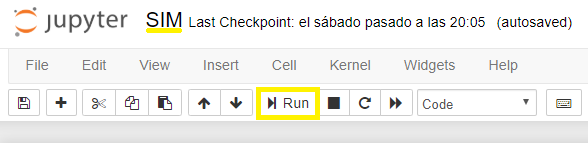
\includegraphics[width=1.1\textwidth]{run}
		\caption{Ejecución de \emph{Jupyter Notebook}}\label{fig:run}
	\end{figure} 

\subsection{Visualización de la BBDD}

Para visualizar la base de datos, únicamente tendremos que arrastrar o abrir el fichero BBDD con \emph{DB Browser}. Como se aprecia en la figura \ref{fig:dbBrowser}, en el apartado \emph{Hoja de datos} se podrá consultar el contenido de nuestras tablas. Asimismo, en el apartado \emph{Estructura} se podrá visualizar el diseño de la BBDD y en el apartado \emph{Ejecutar SQL} se podrán realizar consultas.

\begin{figure}%[!h]
		\centering
		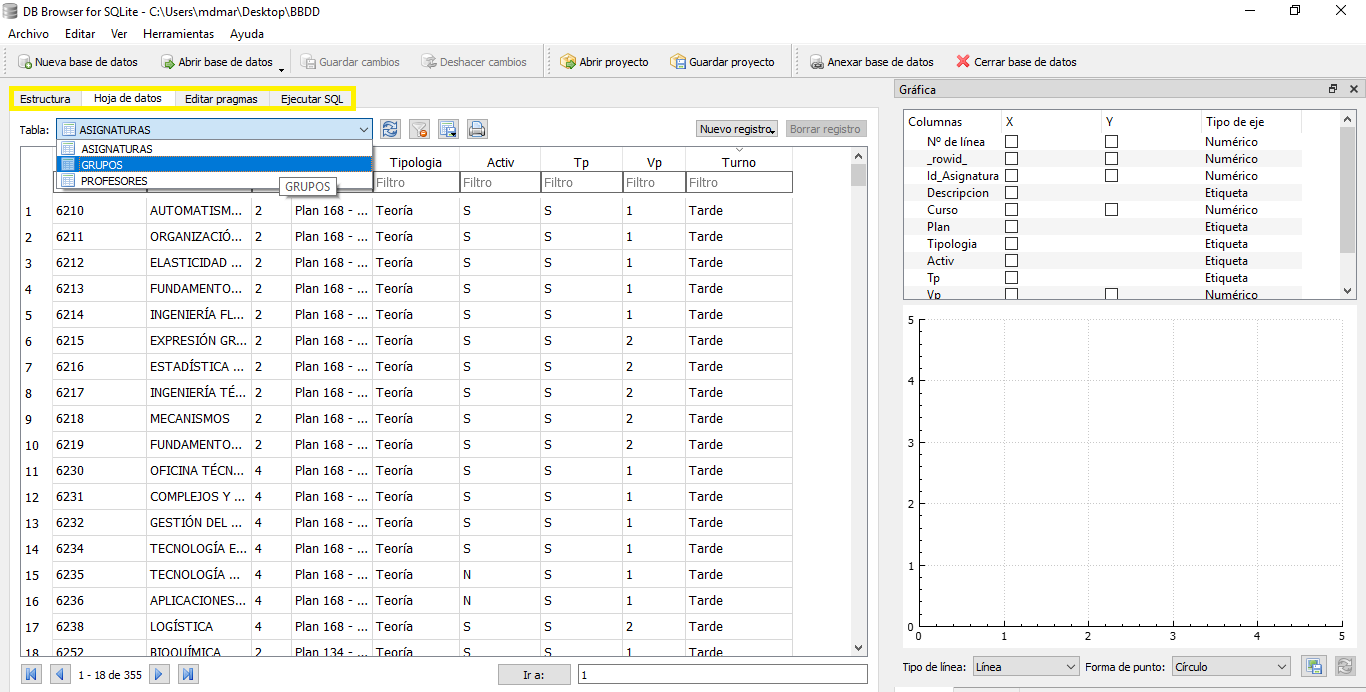
\includegraphics[angle=90, width=0.8\textwidth]{dbBrowser}
		\caption{Ejecución de \emph{Jupyter Notebook}}\label{fig:dbBrowser}
	\end{figure} 











